%!TEX root=ast2016.tex

\begin{figure*}[t]
  \centering
  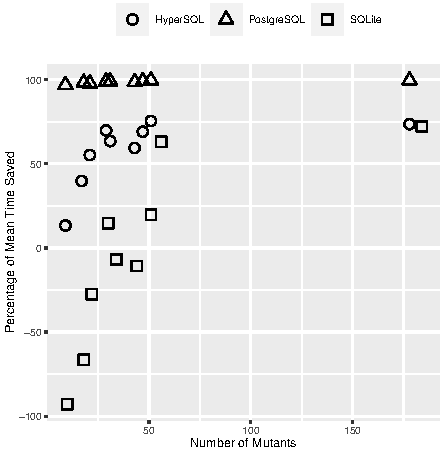
\includegraphics[scale=1.0]{graphics/graphic_scatterplot_nummutants_percentage.pdf}
  \caption{Box plot of the execution time for the original and virtual mutation analysis techniques.}
  \label{fig:graphic_bwplot_schema_analysistime_org_vm}

  % Details about the box plot from the R documentation:

  % The lower and upper "hinges" correspond to the first and third quartiles (the 25th and 75th percentiles). This differs
  % slightly from the method used by the boxplot function, and may be apparent with small samples. See boxplot.stats for for
  % more information on how hinge positions are calculated for boxplot.

  % The upper whisker extends from the hinge to the highest value that is within 1.5 * IQR of the hinge, where IQR is the
  % inter-quartile range, or distance between the first and third quartiles. The lower whisker extends from the hinge to
  % the lowest value within 1.5 * IQR of the hinge. Data beyond the end of the whiskers are outliers and plotted as points
  % (as specified by Tukey).

  % Commentary on the results in this output:

  % - Note that this data has been "log transformed" using a log-to-the-base-ten transformation
  % - Transformation is done because the Postgres-Original data is on a different scale than all other data
  % - This means that you will only see variation for Postgres-Original (without transformation)
  % - Using the log-transformed data shows the basic trends in the data sets

  {\small \justifying{ \noindent In this plot the box itself represents the interquartile range (IQR), or the measure of
      statistical dispersion that is the difference between the first and third quartiles. Furthermore, the upper
      whisker extends from the top of the box to the highest value that is within 1.5 times the IQR, the lower whisker
      goes from the bottom of the box to the lowest value within 1.5 times the IQR, and the thick horizontal line
      represents the median value. The boxes in this plot are noticeably compressed because there is little variance in
      the timings across the different configurations.  Since the results from running the original method on the
      \Postgres DBMS differ substantially from those with the other techniques and databases, all of the
      data values were log-transformed, thereby best revealing the relevant trends.} \par}

\end{figure*}
